\documentclass[10pt,a4paper]{article}
\usepackage[utf8]{inputenc}
\usepackage{amsmath}
\usepackage{amsfonts}
\usepackage{amssymb}
\usepackage{graphicx}
\author{Alberto Lumbreras}
\begin{document}

\begin{itemize}

\item En la ecuación 2, para k=1 (root), tenemos:
\begin{align*}
\delta_{1,t} = 1 + \sum_{m=2}^{t-1} \delta_{1\pi_m}
\end{align*} 

Entonces cuáles son los valores para para $\delta_{0,1}$ y $\delta_{0,2}$? Es decir, cuál es el grado de la raíz cuando llegua el tercer nodo $k=3$ en $t=2$. Para ser consistente con la ecuación 5 donde se asume (lógicamente) que el root no tiene padre, $\delta_{0,1}=0$ y $\delta_{0,2}=1$. Pero entonces, el $1+...$ de la ecuación 2 sobraría para el caso $k=1$, verdad? 

\item En la ecuación 5 calculamos el denominador para el caso de un nuevo nodo en $t+1$ cuyo padre será $\pi_t=k$. El denominador suma las probabilidades asociades a todos los candidatos:
\begin{align*}
Z_t = \alpha\sum_{l=1}^t d_{l,t} + ... = 2\alpha(t-1)
\end{align*}
Esto significa que el número de grados es par dado que toda relación incrementa en uno el grado del padre y del hijo. El grado total es el número de nodos hasta el momento (sin incluir el root) por dos.

\item En la ecuación 8:
\begin{align*}
-\log \mathcal{L}(\Pi | \boldsymbol{\theta}) = - \sum_{i=1}^N \sum_{t=2}^{|\pi_i|} \phi(\pi_{t,i}) - \log \mathbf{Z}_{t,i}
\end{align*}
no falta el $\log$ en $\phi$?

O es que se considera que la función de verosimilitud es:
\begin{align*}
\exp \left\lbrace ad_{k,t} + b_k + \tau^{t-k+1}\right\rbrace
\end{align*}
(entiendo que no ya que decís que si se ignora $b$ se recupera el modelo de Kumar 2010)

\item En la ecuación 8, a diferencia de en vuestro paper de 2011, no sabemos si la función es convexa, no? Qué método usáis para la optimización? Nelder-Mead como en el otro paper?

A la hora de optimizar los parámetros, entiendo que usáis un método que permita establecer máximos y mínimos (ya he visto versiones de Nelder-Mead que lo permiten), en este caso $\alpha \in [0, \infty], \beta \in [0, \infty], \tau \in [0, 1]$ (todos positivos para evitar probabilidades negativas)

\item Para generar los threads artificiales (Sección 3.1), generáis parametros aleatoriamente y para cada conjunto de parámetros generáis 100 conjuntos de N threads cada uno, para así calcular los box plots de la Figura 3. Pero de qué tamaño/s son los threads generados? Entiendo que, como decís en el Apéndice, también elegís el tamaño de la distribución empírica de la Figura 4, verdad? 
\end{itemize}
\begin{figure}
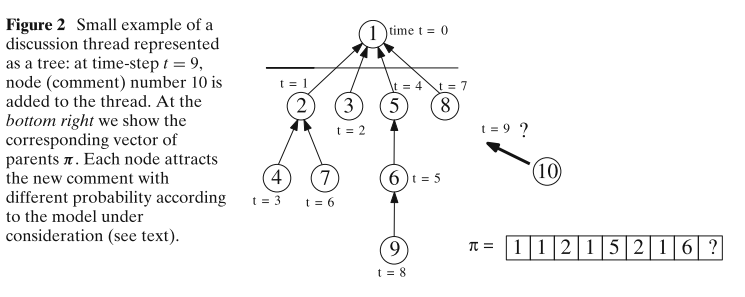
\includegraphics[scale=0.5]{pis}
\end{figure}
\end{document}